\subsubsection{Différences}
	\begin{itemize}
		\item Réalisation de l'inscription automatique au session lors de l'enregistrement de l'utilisateurs. 
		\item Utilisation de type de session afin de facilité et de multiplier le choix des abonnements possible. 
		\item Possibilité pour un utilisateur de s'inscrire à plus de un type de session par semaine. 
		\item Sélection du type de session parmi une liste. 
	\end{itemize}

	\begin{figure*}[h!]
		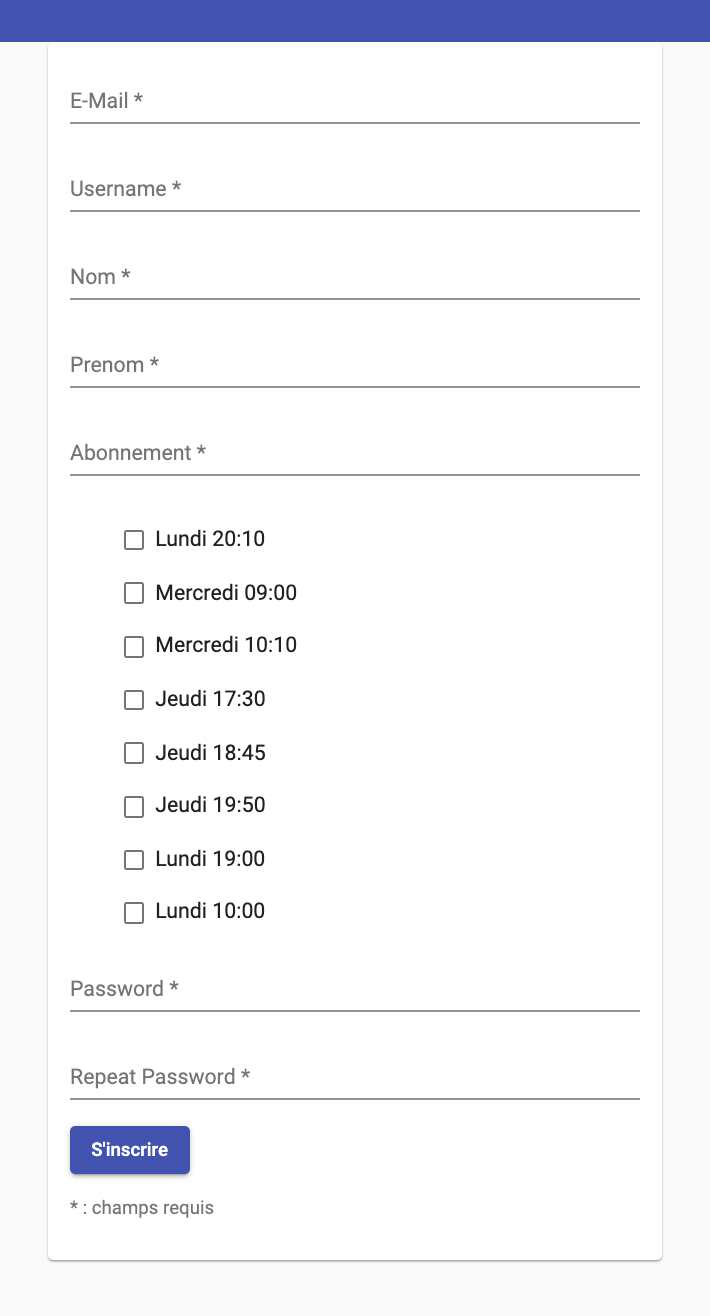
\includegraphics[width = 0.5\textwidth,center]{Figures/us4-1-angular}
		\caption{Formulaire d'inscription version angular}
	\end{figure*}
	
	
\newpage
\subsubsection{Diagramme de séquence}
	\begin{figure}[h]
		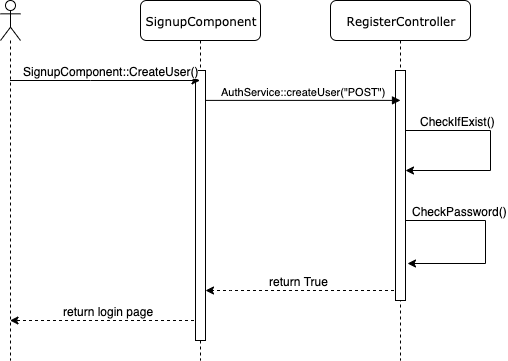
\includegraphics[width=\textwidth,center]{Diagramme/sequence-us1-angular}
		\caption{Diagramme de séquence de l'inscription automatique d'un utilisateur. }
	\end{figure}

\vspace{\baselineskip}
\subsubsection{Script concernés}
	\begin{itemize}
		\item \Href{https://github.com/victorsmits/Aquabike/blob/master/frontend/src/app/service/auth.service.ts}{auth.service.ts}
		\item \Href{https://github.com/victorsmits/Aquabike/blob/master/backend/src/Controller/API/SecurityControllerAPI.php}{SecurityControllerAPI.php}
		\item \Href{https://github.com/victorsmits/Aquabike/blob/master/backend/src/Entity/TypeSession.php}{TypeSession.php}
		\item \Href{https://github.com/victorsmits/Aquabike/blob/master/backend/src/Entity/Session.php}{Session.php}
		\item \Href{https://github.com/victorsmits/Aquabike/blob/master/backend/src/Entity/Inscription.php}{Inscription.php}
		\item \Href{https://github.com/victorsmits/Aquabike/blob/master/backend/src/Entity/Person.php}{Person.php}
		\item \Href{https://github.com/victorsmits/Aquabike/blob/master/frontend/src/app/signup/signup.component.ts}{signup.component.ts}
		\item \Href{https://github.com/victorsmits/Aquabike/blob/master/frontend/src/app/signup/signup.component.html}{signup.component.html}
	\end{itemize}